\documentclass[12pt]{article}
\usepackage{amsmath}
\usepackage{amssymb}
\usepackage{amsthm}
\usepackage{graphicx}
\begin{document}

\begin{flushleft}
Scott Clark \\
MPIPKS
\end{flushleft}

Billiards

\[\Psi_{n,m} = \sqrt{\frac{4}{L_{x}L_{y}}} \sin \left(\frac{n \pi x}{L_{x}} \right) \sin \left(\frac{m \pi y}{L_{y}} \right)\]

\[E \Psi = \frac{- \hbar}{2 m} \left( \frac{\partial^{2} \Psi}{\partial x^{2}} + \frac{\partial^{2} \Psi}{\partial y^{2}} \right)\]

\[E = \frac{\hbar^{2} \pi^{2}}{2 m} \left( \frac{n^{2}}{L_{x}^{2}} + \frac{m^{2}}{L_{y}^{2}} \right)\]

\[\Delta E \Delta t = \hbar \Rightarrow \Delta E = \frac{ \hbar}{\Delta t}\]

\[p = \hbar k = \frac{\hbar 2 \pi}{\lambda} \Rightarrow \frac{\lambda}{p} =  = \Delta t\]

\[E = \frac{p^{2}}{2m} \Rightarrow p = \sqrt{2E}\]

\[\Delta E = \frac{ \sqrt{2E}}{\lambda}\]

\begin{figure}[hpt]
	\centering
		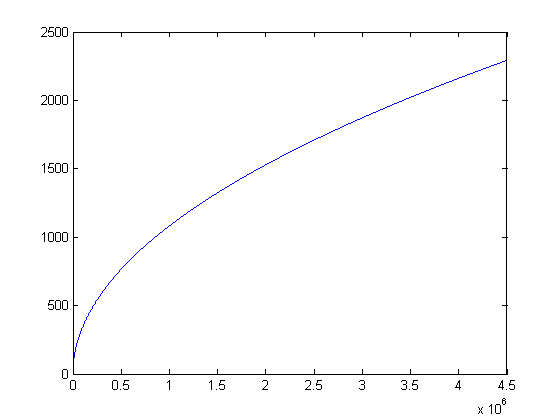
\includegraphics[width=1.00\textwidth]{notes2/EvsDelE.png}
	\caption{Energy with delta E}
	\label{fig:energywdeltaerrors}
\end{figure}

\begin{figure}[hpt]
	\centering
		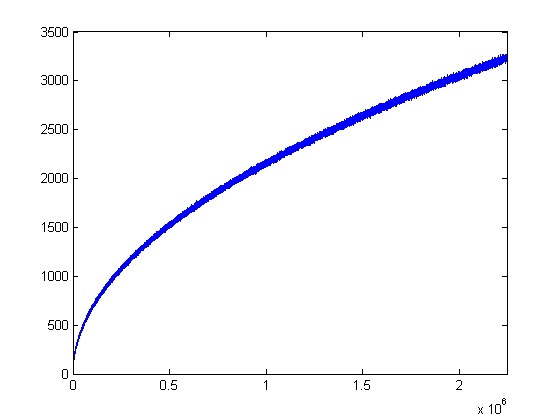
\includegraphics[width=1.00\textwidth]{notes2/EvsNeff.png}
	\caption{Neff for each energy (number of other states within $\Delta$ E of E)}
	\label{fig:neff}
\end{figure}

\begin{figure}[hpt]
	\centering
		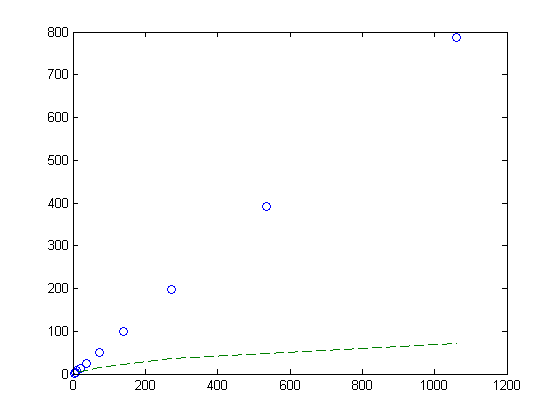
\includegraphics[width=1.00\textwidth]{notes3/nodeavgVsE_deltaEVsE.png}
	\caption{Nodes found 'o' and Neff '--' vs E}
	\label{fig:nodeavgVsE_deltaEVsE}
\end{figure}

\pagebreak

now we plot the distribution of the maximums (for the real case)

\[E = 1061\]
\[\Delta E = 35.1912\]
\[n_{eff} = 72\]
\[n_{maxima} = 787.6230\]
\[\bar{x} = 37.1436\]
\[\sigma = 6.4767\]
\[a = 34.2289\]
\[b = 5.0499\]

\begin{figure}[ht]
	\centering
		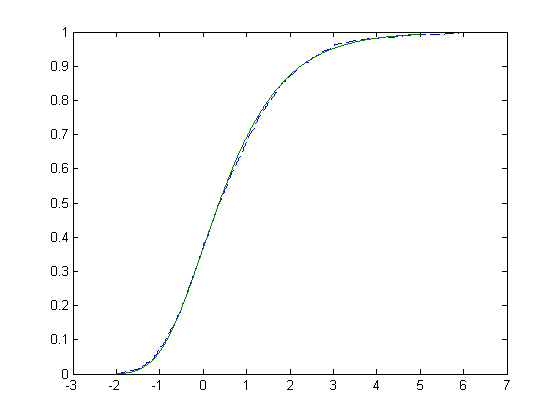
\includegraphics[width=1.00\textwidth]{notes3/gumbel_e2to10.png}
	\caption{Gumbel and distribution of maximums}
	\label{fig:gumbel_e2to10}
\end{figure}

\pagebreak

\[E = 536.2136\]
\[\Delta E = 25.0172\]
\[n_{eff} = 48\]
\[n_{maxima} = 391.6190\]
\[\bar{x} = 27.5574\]
\[\sigma = 5.1807\]
\[a = 25.2259\]
\[b = 4.0394\]

\begin{figure}[hbpt]
	\centering
		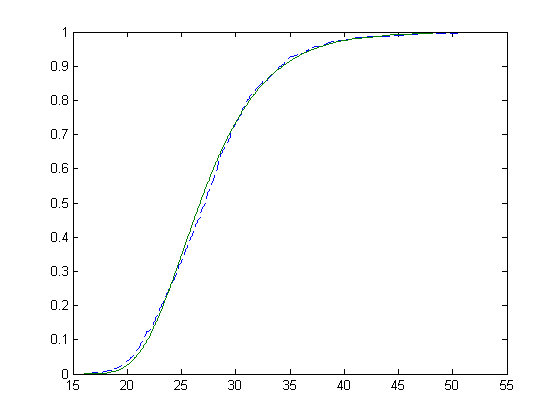
\includegraphics[width=1.00\textwidth]{eg9.png}
	\caption{Gumbel and distribution of maximums}
	\label{fig:eg9}
\end{figure}

\pagebreak

\[E = 273.5530\]
\[\Delta E = 17.8686\]
\[n_{eff} = 36.0000\]
\[n_{maxima} = 198.7900\]
\[\bar{x} = 21.8394\]
\[\sigma = 4.6864\]
\[a = 19.7303\]
\[b = 3.6540\]

\begin{figure}[hbpt]
	\centering
		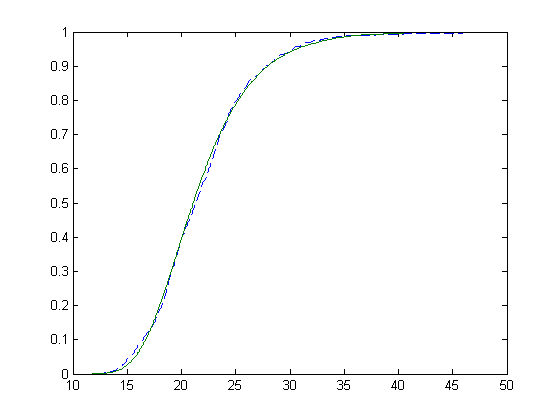
\includegraphics[width=1.00\textwidth]{eg8.png}
	\caption{Gumbel and distribution of maximums}
	\label{fig:eg8}
\end{figure}

\pagebreak

\[E = 140.4477\]
\[\Delta E = 12.8035\]
\[n_{eff} = 22.0000\]
\[n_{maxima} = 99.9460\]
\[\bar{x} = 15.3681\]
\[\sigma = 3.5654\]
\[a = 13.7635\]
\[b = 2.7799\]

\begin{figure}[hbpt]
	\centering
		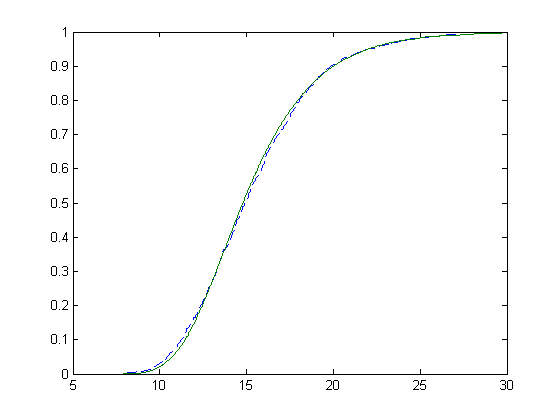
\includegraphics[width=1.00\textwidth]{eg7.png}
	\caption{Gumbel and distribution of maximums}
	\label{fig:eg7}
\end{figure}

\pagebreak

\[E = 73.8885\]
\[\Delta E = 9.2866\]
\[n_{eff} = 16.0000\]
\[n_{maxima} = 50.5520\]
\[\bar{x} = 11.7141\]
\[\sigma = 2.9421\]
\[a = 10.3900\]
\[b = 2.2940\]

\begin{figure}[hbpt]
	\centering
		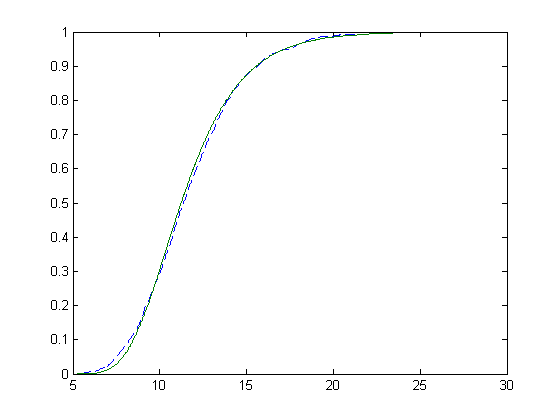
\includegraphics[width=1.00\textwidth]{eg6.png}
	\caption{Gumbel and distribution of maximums}
	\label{fig:eg6}
\end{figure}

\pagebreak

\[E = 38.4721\]
\[\Delta E = 6.7011\]
\[n_{eff} = 9.0000\]
\[n_{maxima} = 25.4700\]
\[\bar{x} = 7.5744\]
\[\sigma = 2.2453\]
\[a = 6.5639\]
\[b = 1.7506\]

\begin{figure}[hbpt]
	\centering
		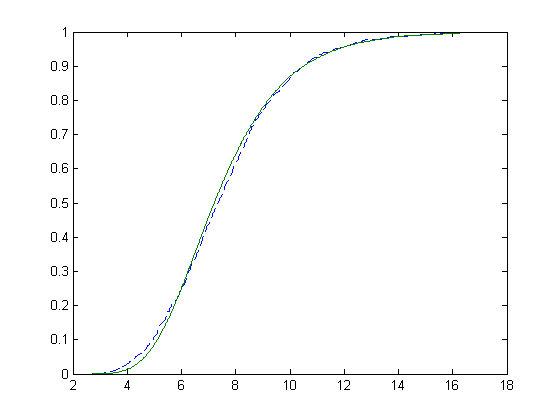
\includegraphics[width=1.00\textwidth]{eg5.png}
	\caption{Gumbel and distribution of maximums}
	\label{fig:eg5}
\end{figure}
\end{document}
